%==============================================================================
\chapter{Metodologia}\label{sec_metodologia}
%==============================================================================

\section{Projeto do Estudo}

\blue{Objetivando mitigar problemas relacionados ao risco de enviesamento por pobreza no relatório sobre o desenvolvimento do modelo \cite{wynants2020prediction}, a metodologia para o desenvolvimento e exposição dos resultados seguem o guia TRIPOD \cite{collins2015tripod}. Este é um \textit{checklist} sobre pontos essenciais que um estudo de diagnóstico ou prognóstico deve relatar quando estiver explanando o desenvolvimento de um modelo preditivo multivariado. O \textit{checklist} TRIPOD deste trabalho pode ser encontrado no apêndice \ref{appendix:tripod}.}

%\section{Participantes}

%\red{O estudo engloba todos os pacientes que foram reportados estado do Rio Grande do Sul que foram reportados pelos dois sistemas de notificações oficiais do Ministério da Saúde no monitoramento da doença: o e-SUS Notifica \cite{instrutivoesus} e o Sistema de Informação da Vigilância Epidemiológica da Gripe (Sivep-Gripe) \cite{instrutivosivep}.} \red{Rio Grande do Sul é um estado localizado ao sul do Brasil, e contém uma população estimada de 11.422.973 pessoas\footnote[4]{https://cidades.ibge.gov.br/brasil/rs/panorama}.}

\section{Participantes}

\red{Para o desenvolvimento, treino e validação do modelo preditivo, utilizamos dados anonimizados provenientes do Painel Coronavírus RS\footnote[3]{https://ti.saude.rs.gov.br/covid19/}. A escolha dos dados foi devido a acessibilidade dos mesmos e também por estarem isentos das leis de proteção aos dados \cite{lgpd2019errc}.} 
\red{Neste estudo, utilizamos um conjunto de dados com 604.389 registros (observações) de casos confirmados de COVID-19. O conjunto de dados original contém um total de 30 variáveis em nível-paciente, incluindo dados demográficos (\textit{e.g.}, sexo e faixa-etária), clínicos (\textit{e.g.}, tosse e dispneia) e temporais (\textit{e.g.}, data do início dos sintomas), compreende o perído de 01 de janeiro de 2021 à 08 de junho de 2021.}

\subsection{Engenharia de características}

\blue{A Figura \ref{figura_data_selection} retrata o fluxo da seleção dos dados elegíveis para este estudo. No conjunto de dados, existem registros de pacientes que vieram a óbito por causas distindas da COVID-19 (20 [ < 0,01\%]), e também há aqueles cujo parecer evolutivo ainda não era conhecido naquele momento, ou seja, que ainda estavam em acompanhamento (17.724 [ < 3\%]).  Há também registros com informação faltante do sintoma dispneia (2.418 [< 0,5]\%). Optamos por remover os registros com informações faltantes e aqueles que não possuem informação relevante para o estudo (\textit{i.e.}, óbitos por outras causas ou em acompanhamento). Ao final da seleção, dos 604.389 registros inicais, 584.228 permaneceram na base para prosseguir o estudo. }

\blue{Além das características iniciais do conjunto de dados\footnote[4]{https://ti.saude.rs.gov.br/covid19/api}, outras seis características foram extraídas do campo textual ``CONDICOES'' (campo pré-existente no conjunto de dados), a saber: cardiopatia, diabetes, doença respiratória, problema renal, obesidade e doença cromossômica.} \blue{Como a variável ``Raça/cor'' possuía 19,98\% (n=116.752) de dados faltantes, sendo estes 58\% dos óbitos totais (n=10.889), e devido ao decréscimo da pontuação do modelo ao adicioná-la como preditora (ver Seção \ref{sec_resultados}), optamos por sua remoção do conjunto de dados.}

\purple{Utilizamos da codificação por rótulo (\textit{label encoding)} nas variáveis pois algoritmos de aprendizagem de máquina performam algebra linear no processo de treinamento \cite{chatfield2011encoding}. Como a distribuição das preditoras é binária, transformamos ``SIM'' para 1 e ``NÃO'' para 0. A única exceção no processo é da variável qualitativa ordinal ``FAIXAETARIA''. Neste caso, cada faixa-etária foi codificada com um número, a saber: ``< 1'': 0; ``01 a 04'': 1; ``05 a 09'': 2; ``10 a 14'': 3; ``15 a 19'': 4; ``20 a 29'': 5, ``30 a 39'': 6; ``40 a 49'': 7; ``50 a 59'': 8; ``60 a 69'': 9; ``70 a 79'': 10; ``80 e mais'': 11.}

\begin{figure}[H]
\caption{Fluxo de seleção dos participantes}
\centering % para centralizarmos a figura
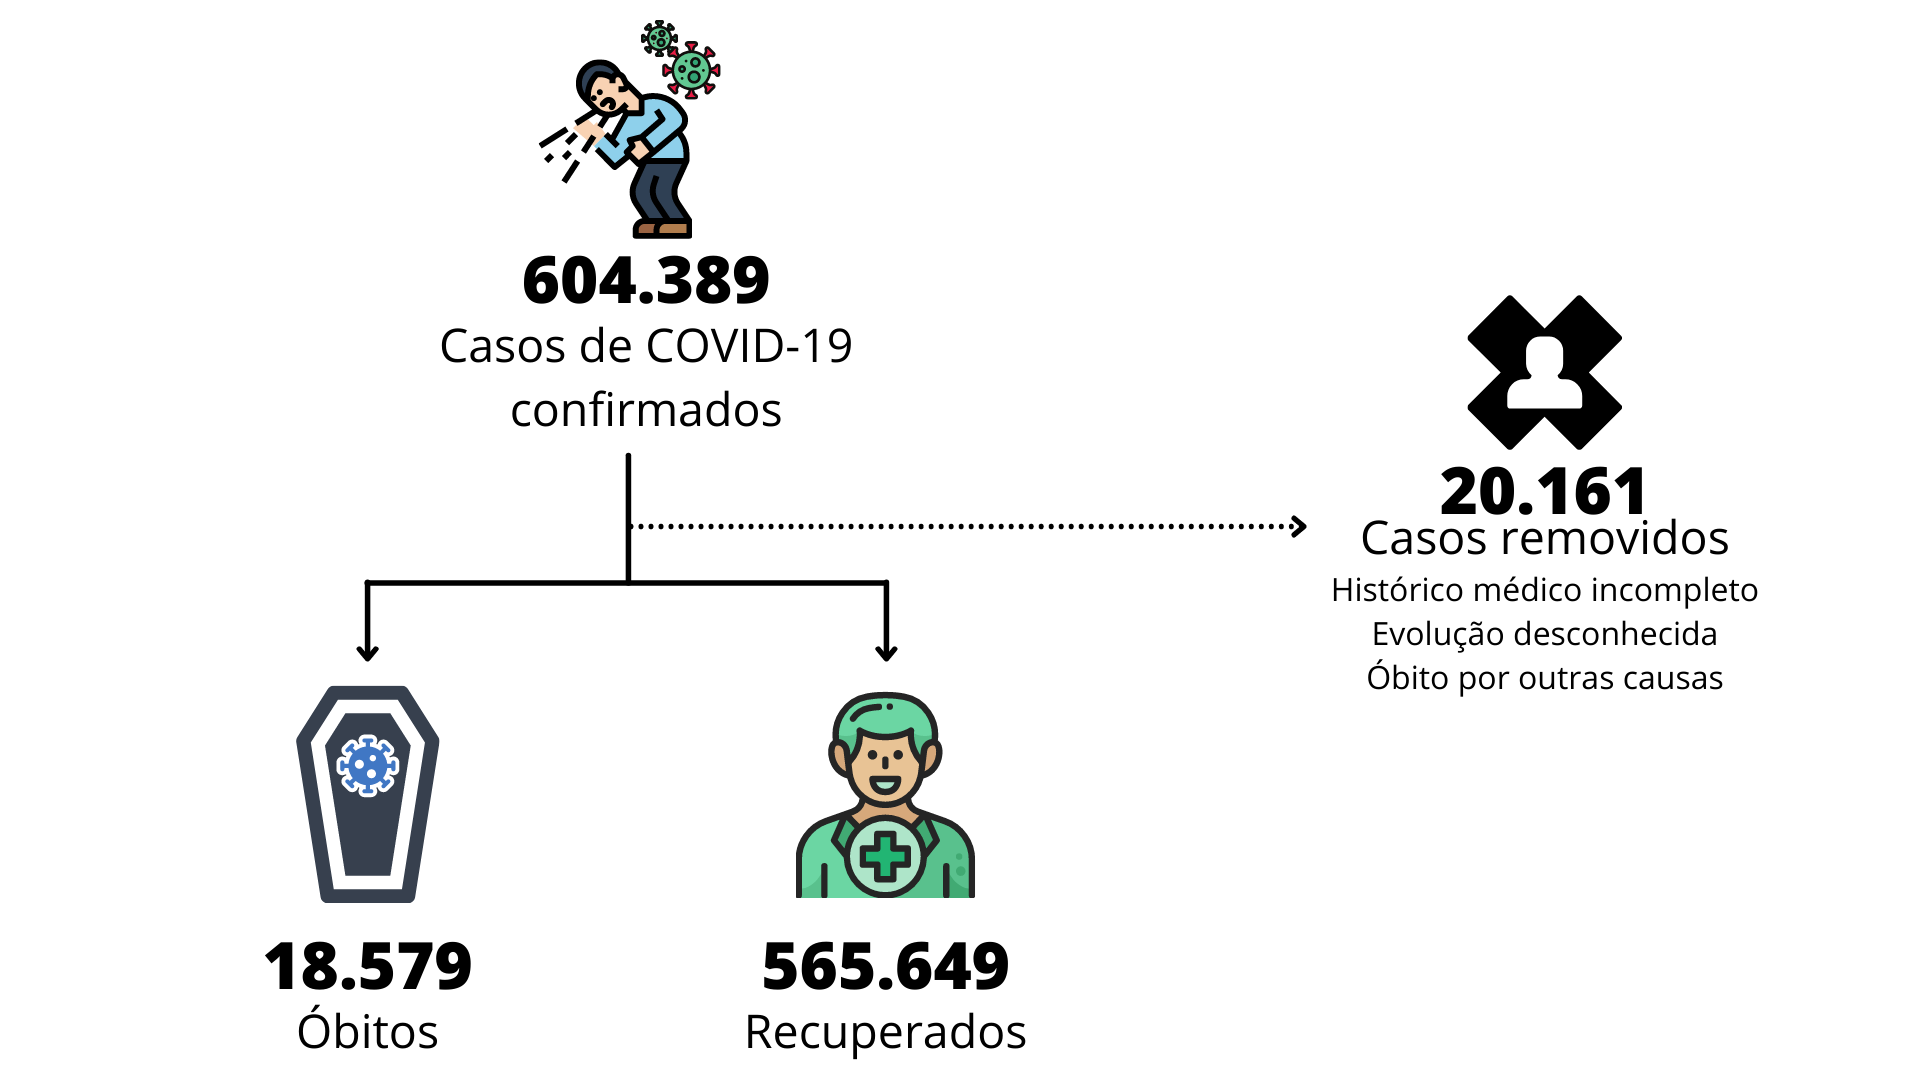
\includegraphics[width=\textwidth]{figuras/fluxo_selecao_participantes.png}
\label{figura_data_selection}
\end{figure}

% variável resposta (dependente) 
\section{Variável resposta}

\red{O principal objetivo do trabalho é prever a chance de óbito entre pacientes positivos de COVID-19. Esta análise prognóstica é importante para a priorização dos pacientes na alocação dos recursos hospitalares. Os dados coletados possuem a informação relacionada a evolução do paciente na variável ``EVOLUCAO''. \purple{Esta variável é dicotômica -- ``ÓBITO'' (1) se o paciente faleceu, e ``RECUPERADO'' (0) caso contrário -- e nos} permite a criação de um modelo de aprendizagem de máquina para classificar os pacientes quanto à sua chance de falecimento, pois informa quais e quantos foram recuperados ou vieram a óbito por COVID-19. }

% variaveis preditoras (independente)
\section{Variáveis Preditoras}

%\blue{Os dados iniciais da base de dados são como segue: a idade dos pacientes é definida em categorias (< 1, 01 a 04, 05 a 09, 10 a 14, 15 a 19, 20 a 29, 30 a 39, 40 a 49, 50 a 59, 60 a 69, 70 a 79, 80 e mais). Raça foi classificada como branca, preta, parda, indígena e amarela. Os sintomas são febre, tosse, garganta, dispneia e a unica condição/comorbidade previamamente existente na base, é a informação sobre gestante. Todos os dados-padrão disponíveis da fonte de dados, podem ser consultados no dicionário de dados disponibilizado pelo Painel Coronavírus RS\footnote[6]{https://ti.saude.rs.gov.br/covid19/api}.}

 \red{As variáveis candidatas para preditoras foram selecionadas baseando-se em um dos critérios comuns \cite{collins2015tripod}: variáveis clínicas conhecidas de diagnóstico comum relacionado a pneumonia ou quadros gripais. Após a extração das novas características e remoção de campos que não são candidatos a variáveis preditoras (\textit{i.e.}, datas e códigos), os dados clínicos, demográficos e categóricos resultantes e que foram utilizados no estudo podem ser vistos na Tabela \ref{tab_dados_limpos}.}


\begin{table}[H]
\caption{Variáveis}
\label{tab_dados_limpos}
\begin{tabular}{lll}
\hline
Nome                  & Descrição                                                                                    & Tipo                   \\ \hline
SEXO                  & Sexo                                                                             & Binária/Demográfica    \\ \hline
FAIXAETARIA           & Faixa etária                                                                     & Categórica/Demográfica \\ \hline
EVOLUCAO              & \begin{tabular}[c]{@{}l@{}}Qual o parecer \\ evolutivo do paciente?\end{tabular}             & Binária/Alvo           \\ \hline
FEBRE                 & Sintomas de febre                                                                   & Binária/Clínica        \\ \hline
TOSSE                 & Sintomas de tosse                                                                   & Binária/Clínica        \\ \hline
GARGANTA              & \begin{tabular}[c]{@{}l@{}}Sintomas de dor de garganta\end{tabular}              & Binária/Clínica        \\ \hline
DISPNEIA              & \begin{tabular}[c]{@{}l@{}}Sintomas de dispnéia/ \\ falta de ar\end{tabular}       & Binária/Clínica        \\ \hline
GESTANTE              & O paciente é gestante?                                                                       & Binária/Clínica        \\ \hline
SRAG                 & \begin{tabular}[c]{@{}l@{}}O quadro clínico se caracteriza \\ como Sindrome Respiratória \\ Aguda Grave?\end{tabular} & Binária/Clínica \\ \hline
CARDIOPATIA           & \begin{tabular}[c]{@{}l@{}}O paciente possui alguma \\ doença cardíaca crônica?\end{tabular} & Binária/Clínica        \\ \hline
DIABETES              & O paciente possui diabetes?                                                                  & Binária/Clínica        \\ \hline
DOENCA\_RESPIRATORIA & \begin{tabular}[c]{@{}l@{}}O paciente possui alguma \\ doença respiratória crônica?\end{tabular}                      & Binária/Clínica \\ \hline
PROBLEMA\_RENAL       & \begin{tabular}[c]{@{}l@{}}O paciente possui \\ problema renal?\end{tabular}                 & Binária/Clínica        \\ \hline
OBESIDADE             & O paciente é obeso?                                                                          & Binária/Clínica        \\ \hline
DOENCA \_CROMOSSOMICA & \begin{tabular}[c]{@{}l@{}}O paciente possui \\ doença cromossômica?\end{tabular}            & Binária/Clínica        \\ \hline
\end{tabular}
\end{table}

% statistical methods
\section{Métodos Estatísticos}

\subsection{Análise descritiva}

\blue{Para entendermos sobre possíveis características que expliquem o risco de óbito, performamos análises descritivas dos preditores por cada grupo e apresentamos os resultados em quantidade e proporção de óbitos. Possíveis correlações foram analisadas utilizando o coeficiente de Pearson \cite{benesty2009pearson} e a importância relativa das características foi analisada através do grau de impureza de Gini \cite{menze2009gini} (\textit{i.e.}, a importância da característica para o modelo).}

\subsection{Análise preditiva}

\blue{Aplicamos um algoritmo de aprendizagem de máquina para prever a chance de óbito entre pacientes confirmados com COVID-19. Para a implementação, análise estatística, avaliação e validação dos modelos, utilizamos a linguagem Python 3, juntamente com as bibliotecas para aprendizagem de máquina: Scikit-learn \cite{pedregosa2011scikit} (floresta aleatória), e de manipulação e visualização de dados Pandas \cite{pandas2010}, Numpy \cite{2020NumPy-Array} e Seaborn \cite{hunter2007matplotlib}.} 

Para garantir a reproducibilidade do experimento, definimos arbritrariamente a semente 777 para embaralhar o conjunto de dados inicial. Utilizamos uma divisão pseudo-aleatória (\textit{random split}) de 70\%/30\%, a partir dos dados iniciais, sendo 70\% utilizado para treinos e testes, e os 30\% restante, para validação interna do modelo \cite{james2013statistical}. 
Avalimamos a performance/discriminação do modelo através da área sobre a curva ROC (AUC-ROC). A pontuação AUC-ROC pode assumir valores de 0 a 1, onde um valor de 0 indica um modelo que erra todas as predições e 1 reflete um teste perfeito de predição. Em geral, um valor de 0,5 sugere que o modelo não tem capacidade de discriminação (\textit{i.e.}, não consegue diferenciar pacientes que vieram a óbito dos recuperados); 0,7 a 0,8 é considerado aceitável; 0,8 a 0,9 é ótimo; e valores acima de 0,9 são considerados excelentes \cite{mandrekar2010receiver}.

Por se tratar de um conjunto de dados desbalanceado, utilizamos da técnica de subamostragem (\textit{under-sampling}, do inglês) para balancear os dados de treino, e então confrontar com o treinamento sem balanceamento para detectar melhorias \cite{anand2010approach}. Esta técnica consiste em selecionar, pseudo-aleatóriamente, pequenas fatias da classe majoritária (recuperado), a fim de igualar à quantidade de dados pertencentes a classe minoritária (óbito). Utilizamos da pesquisa de grade por validação cruzada (\textit{gridsearch cross validation}) para encontrar os melhores hiperparâmetros para o modelo - incluindo a quantidade de árvores de decisão (\texttt{n\_estimators}) e a profundidade máxima de cada árvore (\texttt{max\_depth}) \cite{krstajic2014cross} - que maximizassem a pontuação AUC-ROC nos dados de treino.

\subsection{Validação do modelo}
\blue{Para validação interna do modelo, utilizamos da técnica \textit{K-Fold Cross Validation}, que consiste em dividir o conjunto de dados em K dobras (\textit{folds}). A função de previsão é aprendida usando K-1 dobras, e a dobra deixada de fora é usada para teste. Optamos por utilizar sua variação estratificada (\textit{stratified K-Fold Cross Validation}), ou seja, na adaptação para conjuntos de dados desbalanceados, pois mantém a proporção original de cada classe na etapa de teste.
Geralmente, realiza-se a validação cruzada k-fold usando k = 5 ou k = 10, uma vez que estes valores produzem estimativas de taxa de erro de teste que não sofrem de viés ou variância excessivamente altos \cite{james2013statistical}. Por padrão, a biblioteca Scikit-learn \cite{pedregosa2011scikit} utiliza K = 5, e por isso decidimos manter este valor.}


